%%%%%%%%%%%%%%%%%%%%%%%%%%%%%%%%%%%%%%%%%%%%%%%%%%%%%%%%%%%%%%%%%%%%%%
% Lớp 11 | Hàm số lượng giác và phương trình lượng giác | Hàm số lượng giác và đồ thị
% Dạng 1D1?4-5: Xét tính tuần hoàn, tìm chu kỳ
% Số câu: 42  (sinh tự động bởi tach_cau.py; từ nay thầy sửa trực tiếp file này)
%%%%%%%%%%%%%%%%%%%%%%%%%%%%%%%%%%%%%%%%%%%%%%%%%%%%%%%%%%%%%%%%%%%%%%

%%%%%%%%%%%%%%%% TRẮC NGHIỆM 4 PHƯƠNG ÁN %%%%%%%%%%%%%%%%

% nguồn: Ok_Toan11_TracNghiem_Lan2
\begin{ex}%[1D1N4-5]%[ma:c48b454d]
	Mệnh đề nào sau  đây là $\textbf{sai}$?
	\choice  {Hàm số $y=\tan x$ tuần hoàn với chu kỳ $\pi$}
		{Hàm số $y=\sin x$  tuần hoàn với chu kỳ $2\pi$}
		{Hàm số  $y=\cos x$ tuần hoàn với chu kỳ $2\pi$}
		 {\True Hàm số $y=\cot x$ tuần hoàn với chu kỳ $2\pi$}
	 \loigiai{
		\begin{itemize}
			\item $y = \sin x$, $y = \cos x$ là hai hàm số có chu kì bằng  $2\pi$.
			\item $y=\tan x$, $y=\cot x$ là hai hàm số có chu  kì bằng $\pi$.
		\end{itemize}
	} 
\end{ex}

% nguồn: Ok_Toan11_TracNghiem_Lan2
\begin{ex}%[1D1N4-5]%[ma:775b8d32]
	Trong các hàm số $y=\sin x$, $y=\cos x$, $y=\tan x$, $y=\cot x$ có bao  nhiêu hàm số có chu kì là $2\pi$?
	\choice 
		 {$0$}
		{$1$} 
		{\True  $2$}
		{$3$} 
	 \loigiai{
		\begin{itemize}
			\item $y = \sin x$,  $y = \cos x$ là hai hàm số có chu kì bằng $2\pi$.
			\item $y=\tan x$, $y=\cot x$ là  hai hàm số có chu kì bằng $\pi$.
		\end{itemize}
	 }
\end{ex}

% nguồn: Ok_TracNghiemLop11_Lan1
\begin{ex}%[1D1N4-5]%[ma:94618967]
	Trong các hàm số sau hàm số nào tuần hoàn với chu kỳ $2\pi $. 
	 \choice
		{$y=  \cos 2x$}
		{\True  $y= \sin x$}
		{$y=  \tan 2x$}
		{$y= \cot  2x$}
	\loigiai{ 
		Hàm số  $y=\sin x$ tuần hoàn với chu kì $2 \pi$.
	 }
\end{ex}

% nguồn: Ok_TracNghiemLop11_Lan1
\begin{ex}%[1D1N4-5]%[ma:e1c1fd9f]
	Hãy chỉ ra  hàm số tuần hoàn trong các hàm số sau.
	 \choice
		{$y=x\sin x$} 
		{\True  $y=\sin 3x$}
		{$y=x-\sin  x$}
		 {$y=\dfrac{x}{2+\sin x}$}
	\loigiai{ 
	Hàm số  $y=\sin u(x)$ là hàm tuần hoàn. Vậy $y=\sin 3x$ là hàm tuần hoàn.}
\end{ex}

% nguồn: Ok_TracNghiemLop11_Lan1
\begin{ex}%[1D1N4-5]%[ma:b122c3ce]
	Hàm số $y=\sin 2x$ tuần hoàn với chu kỳ bằng  bao nhiêu?
	 \choice
		 {$T=4\pi $}
		{$T=2\pi  $}
		{\True $T=\pi $} 
		 {$T=\dfrac{\pi }{2}$}
	\loigiai{ 
		Hàm số $y=\sin 2x$ tuần hoàn với chu kỳ bằng $T=\dfrac{2\pi }{2}=\pi  $.
	} 
\end{ex}

% nguồn: Ok_TracNghiemLop11_Lan1
\begin{ex}%[1D1N4-5]%[ma:f5b1d54a]
	Chọn khẳng định  \textbf{sai}.
	\choice 
		 {Hàm số $y=\tan \,x+\sin \,x$ là hàm số tuần hoàn với chu kì $2\pi $}
		{Hàm số $y=\cos  \,x$ là hàm số tuần hoàn với chu kì $2\pi $}
		{Hàm số $y=\cot x+\tan x$  là hàm số tuần hoàn với chu kì $\pi $}
		{\True Hàm số  $y=\sin \,x$ là hàm số tuần hoàn với chu kì $\pi $}
	 \loigiai{
		Hàm số $y=\sin \,x$ và $y=\cos\,x$ tuần hoàn với chu  kì $2\pi $.\\
		Hàm số  $y=\tan \,x$ và $y=\cot\,x$ tuần hoàn với chu kì $\pi $.
	 }
\end{ex}

% nguồn: Ok_Toan11_TracNghiem_Lan2
\begin{ex}%[1D1H4-5]%[ma:b769685c]
	Tìm chu kì $T$ của  hàm số $y=\sin\left(x+\dfrac{\pi}{3}\right)$.
	\choice 
		{$T=\pi$} 
		{$T=4\pi$} 
		{\True $T=2\pi$} 
		 {$T=6\pi$}
	\loigiai{ 
		 Tập xác định là $\mathscr{D}=\mathbb{R}$ nên $\forall x\in \mathscr{D}$ thì $x+2\pi\in \mathscr{D}$ và $x-2\pi\in \mathscr{D}$.\\
		Ta có $y=\sin\left(x+\dfrac{\pi}{3}+2\pi\right)=\sin\left(x+\dfrac{\pi}{3}\right)$.\\ 
		Do  đó $T=2\pi$.
	 }
\end{ex}

% nguồn: Ok_Toan11_TracNghiem_Lan2
\begin{ex}%[1D1H4-5]%[ma:5f7e653c]
	 Hàm số $y = \sin 2x$ có chu kì tuần hoàn là
	 \choice
		 {\True $T = \pi$}
		{$T  = \dfrac{\pi}{2}$}
		 {$T = 4\pi$}
		{$T  = 2\pi$}
	 \loigiai{
		Chu kì tuần hoàn của hàm số $y  = \sin 2x$ là $T = \dfrac{2\pi}{|2|} = \pi$.
	} 
\end{ex}

% nguồn: Ok_Toan11_TracNghiem_Lan2
\begin{ex}%[1D1H4-5]%[ma:1ce0dc59]
	Chu kì của  hàm số $y = 3 + 2\sin^2 2x$ là
	\choice 
		 {\True $\dfrac{\pi}{2}$}
		{$d\frac{\pi}{4}$} 
		 {$\pi$}
		 {$2\pi$}
	\loigiai{ 
		 Ta có $y = 3 + 2\sin^2 2x = 3 + 1 - \cos 4x = 4 - \cos 4x$.\\
		Suy ra chu kì tuần hoàn của hàm  số là $T = \dfrac{2\pi}{4} = \dfrac{\pi}{2}$.
	} 
\end{ex}

% nguồn: Ok_Toan11_TracNghiem_Lan2
\begin{ex}%[1D1H4-5]%[ma:8f1e7d79]
	Tìm chu  kì $T$ của hàm số $y = \cos \left(\dfrac{x}{2} + 2025\right)$.
	 \choice
		{$T =  \pi$}
		{  $T = -2\pi$}
		{\True  $T = 4\pi$}
		{  $T = 2\pi$}
	 \loigiai{
		Hàm số $y = \cos \left(\dfrac{x}{2} + 2025\right)$ tuần hoàn với chu kì $T  = 4\pi$.
	} 
\end{ex}

% nguồn: Ok_Toan11_TracNghiem_Lan2
\begin{ex}%[1D1H4-5]%[ma:6dae87c6]
	Chu kỳ tuần hoàn của hàm số $y=\sin 2x$ là 
	\choice 
		{\True  $\pi$}
		 {$2\pi$}
		 {$\dfrac{\pi}{2}$}
		{$4\pi$} 
	 \loigiai{
		 Ta có $y=\sin 2(x+\pi)=\sin(2x+2\pi)=\sin 2x$.\\
		Do $\pi$ là số dương nhỏ nhất thỏa mãn tính chất trên nên hàm $y=\sin 2x$ tuần hoàn với chu kỳ  $\pi$.
	 }
\end{ex}

% nguồn: Ok_Toan11_TracNghiem_Lan2
\begin{ex}%[1D1H4-5]%[ma:04b27074]
	Chu kỳ của hàm số $y = 3\tan\left(mx+n\right)$ với $m$,  $n$ là những số nguyên dương là
	 \choice
		{\True $\dfrac{\pi}{m}$} 
		{$\dfrac{\pi}{c}$, $c$ là bội  chung nhỏ nhất của $m$, $n$}
		{$\dfrac{\pi}{mn}$} 
		{$\dfrac{\pi}{d}$, $d$ là ước  chung lớn nhất của $m$, $n$}
	 \loigiai{
		Ta có chu kỳ của hàm số $y = 3\tan(mx+n)$  là $\dfrac{\pi}{|m|} = \dfrac{\pi}{m}$.
	} 
\end{ex}

% nguồn: Ok_Toan11_TracNghiem_Lan2
\begin{ex}%[1D1H4-5]%[ma:32502f7f]
	Tìm chu kì $T$ của hàm số $y = \tan  \left(2x - \dfrac{\pi}{3}\right)$.
	\choice 
		{$k2\pi$,  $k \in \mathbb{Z}$}
		 {\True $\dfrac{\pi}{2}$}
		 { $\pi$}
		{  $2\pi$}
	\loigiai{ 
		Hàm số $y =  \tan \left(2x - \dfrac{\pi}{3}\right)$ tuần hoàn với chu kì $T = \dfrac{\pi}{2}$.
	} 
\end{ex}

% nguồn: Ok_Toan11_TracNghiem_Lan2
\begin{ex}%[1D1H4-5]%[ma:78baf350]
	Hàm số $y = \sin 2x + \cos \left(3x +  \dfrac{\pi}{4}\right)$ có chu kì là
	 \choice
		{$3\pi$} 
		{\True $2\pi$} 
		{$\frac{\pi}{6}$} 
		{$6\pi$} 
	 \loigiai{
		Ta thấy $\sin 2x$ có chu kì $T_1 = \dfrac{2\pi}{2} = \pi$, $\cos \left(3x + \dfrac{\pi}{4}\right)$ có chu kì  $T_2 = \dfrac{2\pi}{3}$.\\
		Vì hàm số $y = \sin 2x +  \cos \left(3x + \dfrac{\pi}{4}\right)$ là tổng của hai hàm trên nên chu kì của $y$ là bội chung nhỏ nhất của $T_1$ và $T_2$.\\
		Vậy hàm số $y = \sin 2x + \cos \left(3x + \dfrac{\pi}{4}\right)$ có chu  kì $T = 2\pi$.
	 }
\end{ex}

% nguồn: Ok_TracNghiemLop11_Lan1
\begin{ex}%[1D1H4-5]%[ma:dd81ccd8]
	Mệnh đề nào sau đây  \textbf{sai}?
	 \choice
		{Hàm số xác  định trên tập số thực là hàm số $y=\dfrac{\cos x+\sin x+3}{\sin 3x+\cos 3x+3}$}
		{\True Hàm số lượng giác là hàm tuần hoàn với chu kỳ  $2\pi $}
		{Hàm số có chu kỳ là $\pi $ là hàm số $y=\sin 2x+\tan x+{{\cos }^2}x$} 
		{Phương trình $\tan  x=\sqrt{3}$ có $2$ nghiệm thuộc vào $\left( -3;3 \right)$}
	\loigiai{ 
		Phương trình  $\sin 3x+\cos 3x+3=0$ vô nghiệm nên hàm số có tập xác định là $\mathbb{R}$.\\
		Hàm $y=\tan x$  có chu kỳ là $\pi $.\\
		Hàm số $y=\sin 2x+\tan  x+{{\cos }^2}x$ có chu kỳ là $\pi $.\\
	Phương trình $\tan x=\sqrt{3}$  có $2$ nghiệm $x=\pm \dfrac{\pi }{3}$ thuộc khoảng $\left( -3;3 \right)$.}
\end{ex}

% nguồn: Ok_Toan11_TracNghiem_Lan2
\begin{ex}%[1D1V4-5]%[ma:d2490f3b]
	 Hàm số $y = \tan \left(\dfrac{x}{3} + \dfrac{\pi}{4}\right)$ là hàm số tuần hoàn với chu kỳ bằng
	 \choice
		{$4\pi$} 
		{\True $3\pi$} 
		{$2\pi$} 
		{$6\pi$} 
	 \loigiai{
		Hàm số $y = \tan\left(\dfrac{x}{3} + \dfrac{\pi}{4}\right)$ có tập xác định $\mathscr{D} = \mathbb{R} \setminus \left\{\dfrac{3\pi}{4} +  k3\pi, k \in \mathbb{Z}\right\}$.\\
		Giả sử hàm số tuần hoàn  với chu kỳ $T>0$.\\
		Khi  đó
		$$f(x+T) = f(x), \forall x \in \mathscr{D} \Leftrightarrow  \tan\left(\dfrac{x+T}{3} + \dfrac{\pi}{4}\right) = \tan\left(\dfrac{x}{3} + \dfrac{\pi}{4}\right), \forall x \in \mathscr{D}.$$
		Chọn $x = -\dfrac{3\pi}{4}$, ta được $\tan\left(\dfrac{T}{3}\right) = 0 \Leftrightarrow \dfrac{T}{3} = k\pi \Leftrightarrow T = k3\pi$, $k \in \mathbb{Z}$.\\ 
		 Thử lại ta được $\forall x \in \mathscr{D}$, $f(x+T) = f(x)$ và $x+3\pi$, $x-3\pi \in \mathscr{D}$.\\
		Với $k=1$, ta được $T = 3\pi$ là số dương bé nhất thỏa mãn  nên hàm số tuần hoàn chu kì $T = 3\pi$.
	 }
\end{ex}


%%%%%%%%%%%%%%%% ĐÚNG/SAI %%%%%%%%%%%%%%%%

% nguồn: Ok_dungsai_lop11_Lan1
\begin{ex}%[1D1N4-5]%[ma:c819e4ba]
 Mỗi khẳng định dưới  đây đúng hay sai?
 \choiceTF 
   {\True Hàm số $y=\tan x$ là hàm số tuần hoàn với chu kỳ là $\pi$}
  {\True Hàm số $y=\cos x$ là hàm số tuần hoàn với chu kỳ là  $2 \pi$}
  {Hàm số $y=\sin x$ là hàm số tuần hoàn với chu kỳ là $\pi$} 
  {\True Hàm số $y=\cot  x$ là hàm số tuần hoàn với chu kỳ là $\pi$}
 \loigiai{ 
  \begin{itemchoice}
   \itemch Hàm số $y=\tan x$ là hàm số tuần hoàn với chu kỳ  là $\pi$.
   \itemch Hàm số $y=\cos x$ là hàm số tuần hoàn với chu kỳ là $2 \pi$. 
   \itemch Hàm số  $y=\sin x$ là hàm số tuần hoàn với chu kỳ là $2\pi$.
   \itemch Hàm  số $y=\cot x$ là hàm số tuần hoàn với chu kỳ là $\pi$.
  \end{itemchoice}
  }
\end{ex}

% nguồn: Ok_dungsai_lop11_Lan1
\begin{ex}%[1D1N4-5]%[ma:48198fb5]
 Cho các hàm số $f(x)=\sqrt{3-2\sin x}$; và $g(x)=\tan \dfrac{x}{2}-\dfrac{1}{3}  \cos x$, khi đó:
 \choiceTF 
  {\True Hàm số $f(x)$ có tập  xác định là $\mathscr{D}=\mathbb{R}$}
  {\True Hàm số $f(x)$ đã cho  là hàm tuần hoàn}
  {Hàm số  $g(x)$ xác định khi $x\ne k2\pi, (k\in \mathbb{Z})$}
   {Hàm số $g(x)$ đã cho là hàm không tuần hoàn}
 \loigiai{ 
  \begin{itemchoice}
   \itemch Đúng. Hàm số xác định  $\Leftrightarrow 3-2\sin x\ge 0\Leftrightarrow \sin x\le \dfrac{3}{2}$ (đúng với mọi $x\in \mathbb{R}$).
   Vì vậy tập xác  định hàm số là $\mathscr{D}=\mathbb{R}$.
   \itemch Đúng. Với mọi  $x\in \mathscr{D}$ thì $x\pm 2\pi \in \mathscr{D}$ và $$f(x+2\pi)=\sqrt{3-2\sin (x+2\pi)}=\sqrt{3-2\sin x}=f(x).$$
    Vậy hàm số đã cho là hàm tuần hoàn.
   \itemch Sai. Hàm số xác định $\Leftrightarrow \cos \dfrac{x}{2} \ne 0\Leftrightarrow \dfrac{x}{2} \ne \dfrac{\pi}{2}+k\pi, (k\in \mathbb{Z})\Leftrightarrow x\ne \pi+k2\pi (k\in \mathbb{Z})$. 
   Vì vậy tập xác định hàm số là $\mathscr{D}=\mathbb{R}\setminus \{\pi+k2\pi k\in  \mathbb{Z}\}$.
   \itemch Sai. Với mọi $x\in \mathscr{D}$ thì  $x\pm 2\pi \in \mathscr{D}$ và
   \[\begin{array}{ll}{f(x+2\pi)} & {=\tan \dfrac{x+2\pi}{2}-\dfrac{1}{3} \cos (x+2\pi)} \\ {} & {=\tan \left(\dfrac{x}{2}+\pi \right)-\dfrac{1}{3} \cos x=\tan \dfrac{x}{2}-\dfrac{1}{3} \cos x=f(x).}
  \end{array}
  \] 
  Vậy hàm số đã  cho là hàm tuần hoàn.
 \end{itemchoice}
 }
\end{ex}

% nguồn: Ok_dungsai_lop11_Lan1
\begin{ex}%[1D1N4-5]%[ma:9fd9b52a]
 Cho hàm số $y=f(x)$ xác định trên $\mathbb{R}$ và  có đồ thị như hình vẽ sau
 \begin{center}
  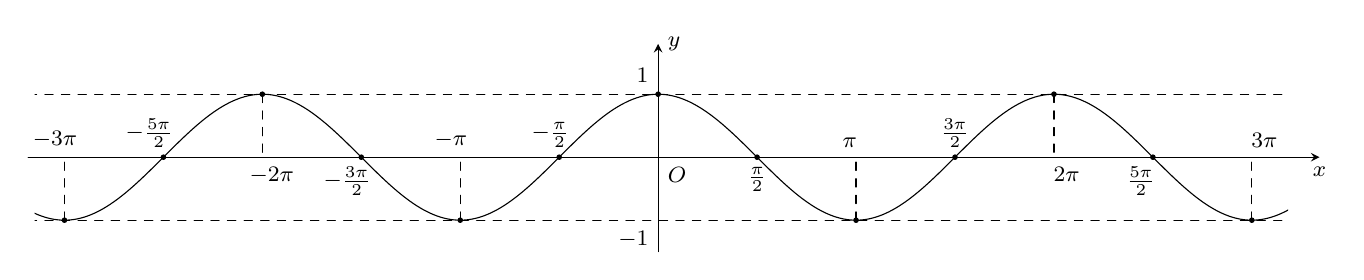
\begin{tikzpicture}[scale=0.8,>=stealth,font=\footnotesize,line join=round,line cap=round]
    \def\xmin{-10}  \def\xmax{10.5} \def\ymin{-1.5} \def\ymax{1.8}
    \draw[->]  (\xmin,0)--(\xmax,0) node [below]{$x$};
    \draw[->]  (0,\ymin)--(0,\ymax) node [right]{$y$};
    \node at (0,0) [below  right]{$O$};
    \clip (\xmin+0.1,\ymin+0.1) rectangle (\xmax-0.5,\ymax-0.1); 
     \draw[smooth,samples=400,domain=\xmin:\xmax] plot (\x,{cos (\x r)});
    \draw[dashed]  (\xmin,1)--(\xmax,1)
     (\xmin,-1)--(\xmax,-1); 
    \foreach \x  in {-3*pi,-2.5*pi,-2*pi,-1.5*pi,-pi,-0.5*pi,0}
     {\draw[fill=black] (\x,cos \x*180/pi) circle (1pt); 
     \draw[dashed] (\x,cos \x*180/pi)--(\x,0);
    \draw[fill=black] (-\x,cos  -\x*180/pi) circle (1pt);
    \draw[dashed] (-\x,cos  \x*180/pi)--(-\x,0);}
     \node at (0,1.3) [left]{$1$};
    \node at  (0,-1.3) [left]{$-1$};
    \node  at (-2*pi+0.15,0) [below]{$-2\pi$};
    \node  at (-3*pi-0.15,0) [above]{$-3\pi$};
    \node at (-2.4*pi,0)  [above left]{$-\frac{5\pi}{2}$};
    \node  at (-1.4*pi,0) [below left]{$-\frac{3\pi}{2}$};
    \node at  (-pi-0.15,0) [above]{$-\pi$};
    \node  at (-0.4*pi,0) [above left]{$-\frac{\pi}{2}$};
     \node at (0.5*pi,0) [below]{$\frac{\pi}{2}$};
     \node at (pi-0.1,0) [above]{$\pi$};
    \node  at (1.5*pi,0) [above]{$\frac{3\pi}{2}$};
     \node at (2*pi+0.2,0) [below]{$2\pi$};
    \node  at (2.5*pi+0.2,0) [below left]{$\frac{5\pi}{2}$};
    \node at (3*pi+0.2,0) [above]{$3\pi$}; 
   \end{tikzpicture}
 \end{center}
 Mỗi khẳng định sau đây  đúng hay sai?
 \choiceTF 
   {Hàm số $y=f(x)$ là hàm số tuần hoàn với chu kỳ là $\dfrac{\pi}{2}$}
  { Hàm số $y=f(x)$ là hàm số tuần hoàn  với chu kỳ là $\pi$}
  {\True Hàm số $y=f(x)$ là hàm số  tuần hoàn với chu kỳ là $2\pi$}
  {Hàm số $y=f(x)$ là hàm số tuần hoàn với chu kỳ  là $\dfrac{3\pi}{2}$}
 \loigiai{Dựa vào đồ thị ta thấy hàm số $y=f(x)$  là hàm số tuần hoàn với chu kỳ là $2\pi$.}
\end{ex}

% nguồn: Ok_dungsai_lop11_Lan2
\begin{ex}%[1D1N4-5]%[ma:6556eea8]
	Cho hàm số $y=\sin x$.  Khi đó
	 \choiceTF{\True Hàm số đã cho có tập xác định là $\mathbb{R}$}
		{Hàm số  đã cho có tập giá trị là $\mathbb{R}$}
		{Hàm số đã cho  là hàm số chẵn}
		{Hàm số đã cho là  hàm số tuần hoàn với chu kỳ $\pi$}
	\loigiai{ 
		\begin{itemchoice}
			 \itemch \textbf{Đúng.}\\
			Hàm số  đã cho có tập xác định là $\mathbb{R}$.
			 \itemch \textbf{Sai.}\\
			Hàm  số đã cho có tập giá trị là $\left[-1; 1\right]$.
			 \itemch \textbf{Sai.}\\
			Hàm số đã cho  là hàm số lẻ.
			\itemch  \textbf{Sai.}\\
			Hàm số đã cho là hàm  số tuần hoàn với chu kỳ $2\pi$.
		\end{itemchoice}
	 }
\end{ex}

% nguồn: Ok_dungsai_lop11_Lan2
\begin{ex}%[1D1H4-5]%[ma:fa9e711d]
	Cho hàm số $f(x)=2\cos x+1$ và $g(x)=\sin x+\tan  x$. Khi đó
	\choiceTF{\True Tập xác định hàm số $f(x)$ là  $\mathscr{D}=\mathbb{R}$}
		{\True Hàm số  $f(x)$ là hàm tuần hoàn}
		{Tập xác định hàm số $g(x)$ $\mathscr{D}=\mathbb{R}\setminus \left\{\dfrac{\pi}{3}+k\pi \mid k\in \mathbb{Z}\right\}$} 
		{Hàm số $g(x)$ là hàm không tuần  hoàn}
	 \loigiai{
		\begin{itemchoice}
			\itemch \textbf{Đúng.}\\ 
			Tập xác định hàm số  $\mathscr{D}=\mathbb{R}$.
			\itemch  \textbf{Đúng.}\\
			Với mọi  $x\in \mathscr{D}$ thì $x\pm 2\pi \in \mathscr{D}$ và $f(x+2\pi)=2\cos (x+2\pi)+1=2\cos x+1=f(x)$. \\
			Vậy hàm số  đã cho là hàm tuần hoàn.
			\itemch \textbf{Sai.}\\ 
			Tập  xác định hàm số $g(x)$ là $\mathscr{D}=\mathbb{R}\setminus \left\{\dfrac{\pi}{2}+k\pi \mid k\in \mathbb{Z}\right\}$.
			\itemch  \textbf{Sai.}\\
			Với mọi $x\in \mathscr{D}$ thì $x\pm 2\pi  \in \mathscr{D}$ và $f(x+2\pi)=\sin (x+2\pi)+\tan (x+2\pi)=\sin x+\tan x=f(x)$. \\
			Vậy hàm số  $g(x)$ đã cho là hàm tuần hoàn.
		\end{itemchoice}
	 }
\end{ex}

% nguồn: Ok_dungsai_lop11_Lan2
\begin{ex}%[1D1H4-5]%[ma:e01f5157]
	Hình bên vẽ đồ thị $y=\sin x$.  Khi đó
	\begin{center}
		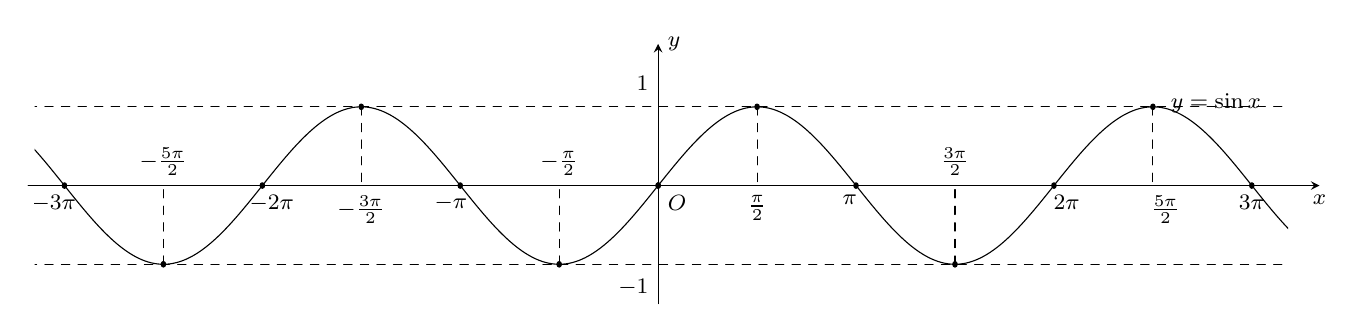
\begin{tikzpicture}[xscale=0.8,>=stealth,font=\footnotesize,line join=round,line cap=round]
				\def\xmin{-10} \def\xmax{10.5}  \def\ymin{-1.5} \def\ymax{1.8}
				\draw[->] (\xmin,0)--(\xmax,0)  node [below]{$x$};
				\draw[->] (0,\ymin)--(0,\ymax) node [right]{$y$}; 
				 \node at (0,0) [below right]{$O$};
				\clip (\xmin+0.1,\ymin+0.1) rectangle (\xmax-0.5,\ymax-0.1); 
				\draw[smooth,samples=400,domain=\xmin:\xmax] plot (\x,{sin (\x r)}); 
				\draw[dashed]  (\xmin,1)--(\xmax,1)
					(\xmin,-1)--(\xmax,-1); 
				\foreach \x  in {-3*pi,-2.5*pi,-2*pi,-1.5*pi,-pi,-0.5*pi,0}
					{\draw[fill=black] (\x,sin \x*180/pi) circle  (1pt);
				 \draw[dashed] (\x,sin \x*180/pi)--(\x,0);
				\draw[fill=black]  (-\x,sin -\x*180/pi) circle (1pt);
				 \draw[dashed] (-\x,sin -\x*180/pi)--(-\x,0);}
				\node at  (0,1.3) [left]{$1$};
				 \node at (0,-1.3) [left]{$-1$};
				\node at (-2*pi+0.15,0) [below]{$-2\pi$}; 
				\node at  (-3*pi-0.17,0) [below]{$-3\pi$};
				 \node at (-2.5*pi,0) [above]{$-\frac{5\pi}{2}$};
				\node at  (-1.5*pi,0) [below]{$-\frac{3\pi}{2}$};
				\node  at (-pi-0.15,0) [below]{$-\pi$};
				\node at (-0.5*pi,0) [above]{$-\frac{\pi}{2}$}; 
				\node at (0.5*pi,0) [below]{$\frac{\pi}{2}$}; 
				\node at (pi-0.1,0)  [below]{$\pi$};
				\node  at (1.5*pi,0) [above]{$\frac{3\pi}{2}$};
				\node  at (2*pi+0.2,0) [below]{$2\pi$};
				\node at (2.5*pi+0.2,0) [below]{$\frac{5\pi}{2}$}; 
				\node  at (3*pi,0) [below]{$3\pi$};
				\node at (2.5*pi+1,0.8) [above]{$y=\sin x$}; 
			\end{tikzpicture}
	\end{center}
	 \choiceTF
		{Hàm số trên là hàm số chẵn, đối xứng  qua trục $Oy$}
		{\True Hàm số trên tuần  hoàn với chu kì $2\pi$}
		{Hàm số nghịch biến trên khoảng $\left(-\dfrac{5\pi}{2};  \;-\dfrac{3\pi}{2}\right)$}
		{\True Trong khoảng từ $-\dfrac{5\pi}{6}$ đến $\dfrac{7\pi}{6}$,  $\sin x\ge \dfrac{1}{2}$ khi và chỉ khi $\dfrac{\pi}{6}\le x\le \dfrac{5\pi}{6}$}
	 \loigiai{
		\begin{itemchoice}
			\itemch  \textbf{Sai.}\\
			Hàm số $y=\sin x\;$  là hàm số lẻ, có đồ thị đối xứng qua gốc toạ độ $O$.
			\itemch \textbf{Đúng.}\\ 
			Hàm số $y=\sin x, y=\cos x$ tuần hoàn với chu kì $2\pi$. Hàm số $y=\tan x, \; y=\cot x$ tuần hoàn với chu kì  $\pi$.
			\itemch  \textbf{Sai.}\\
			Trên khoảng $\left(-\dfrac{5\pi}{2}; \;-\dfrac{3\pi}{2}\right)$ đồ thị  có chiều hướng đi lên, nên hàm số đồng biến.
			 \itemch \textbf{Đúng.}\\
			Xét hàm số $y=\sin x$ trên đoạn $\left[-\dfrac{5\pi}{6}; \dfrac{7\pi}{6}\right]$.  \\
			Ta thấy $\sin x\ge \dfrac{1}{2}$ khi  và chỉ khi $\dfrac{\pi}{6}\le x\le \dfrac{5\pi}{6}$.
		\end{itemchoice}
	} 
\end{ex}

% nguồn: Ok_dungsai_lop11_Lan2
\begin{ex}%[1D1H4-5]%[ma:97b74a5f]
	 Cho hàm số $y=\sqrt{2}\cos \left(2x+\dfrac{\pi}{4}\right)+\sin \left(2x-\dfrac{\pi}{2}\right)$. Khi đó
	 \choiceTF{\True Tập xác định của hàm số là $\mathbb{R}$}
		{Rút  gọn biểu thức ta được $y=\sin 2x$}
		{\True Hàm số tuần hoàn với  chu kì $\pi$}
		{Nếu $\sqrt{2}\cos \left(2x+\dfrac{\pi}{4}\right)+\sin \left(2x-\dfrac{\pi}{2}\right)=-\dfrac{1}{3}$ thì giá trị biểu thức $P=\dfrac{2\tan 2x+\cot 2x}{4\tan 2x-3\cot  2x}$ là $\dfrac{5}{14}$}
	 \loigiai{
		\begin{itemchoice}
			 \itemch \textbf{Đúng.}\\
			Hàm số  có tập xác định của hàm số là $\mathbb{R}$.
			 \itemch \textbf{Sai.}\\
			 Ta có
			\[y=\sqrt{2}\cos \left(2x+\dfrac{\pi}{4}\right)+\sin \left(2x-\dfrac{\pi}{2}\right)=\sqrt{2}\cdot\dfrac{\sqrt{2}}{2}\left(\cos 2x-\sin  2x\right)-\cos 2x=-\sin 2x. \]
			\itemch  \textbf{Đúng.}\\
			Ta có 
			\[y=f(x)=\sqrt{2}\cos  \left(2x+\dfrac{\pi}{4}\right)+\sin \left(2x-\dfrac{\pi}{2}\right)=\sqrt{2}\cdot\dfrac{\sqrt{2}}{2}\left(\cos 2x-\sin 2x\right)-\cos 2x=-\sin 2x. \]
			\begin{itemize}
				\item Tập xác  định $D=R$.
				\item $x+\pi \in \mathscr{D}$ và $x-\pi \in \mathscr{D}$, $\forall x\in  \mathscr{D}$.
				\item $f\left(x+\pi \right)=-\sin 2\left(x+\pi \right)=-\sin 2x=f(x),  \forall x\in \mathscr{D}$.
			\end{itemize}
			Vậy hàm số $y=\sqrt{2}\cos \left(2x+\dfrac{\pi}{4}\right)+\sin \left(2x-\dfrac{\pi}{2}\right)=-\sin 2x$ là hàm số  tuần hoàn với chu kì $\pi$.
			\itemch  \textbf{Sai.}\\
			Ta có $\sqrt{2}\cos \left(2x+\dfrac{\pi}{4}\right)+\sin \left(2x-\dfrac{\pi}{2}\right)=-\dfrac{1}{3}\Leftrightarrow-\sin 2x=-\dfrac{1}{3}$. 
			\[P=\dfrac{2\tan 2x+\cot  2x}{4\tan 2x-3\cot 2x}=\dfrac{2\cdot\dfrac{\sin 2x}{\cos 2x}+\dfrac{\cos 2x}{\sin 2x}}{4\cdot\dfrac{\sin 2x}{\cos 2x}-3\dfrac{\cos 2x}{\sin 2x}}=\dfrac{2\sin^22x+\cos^22x}{4\sin^22x-3\cos^22x}=\dfrac{2\cdot\dfrac{1}{9}+\dfrac{8}{9}}{4\cdot\dfrac{1}{9}-3\cdot\dfrac{8}{9}}=-\dfrac{1}{2}. \]
		\end{itemchoice}
	 }
\end{ex}

% nguồn: Ok_dungsai_lop11_Lan2
\begin{ex}%[1D1H4-5]%[ma:0a2963a7]
	Cho các hàm số  $f(x)=\sqrt{3-2\sin x}$ và $g(x)=\tan\dfrac{x}{2}-\dfrac{1}{3}\cos x$. Xét tính đúng sai của các khẳng định sau
	 \choiceTF
		{\True Hàm số $f(x)$  có tập xác định là $\mathscr{D}=\mathbb{R}$}
		{\True Hàm số $f(x)$ đã cho là  hàm tuần hoàn}
		{Hàm số $g(x)$ xác định khi $x \ne k2\pi$  ($k \in \mathbb{Z}$)}
		{Hàm số $g(x)$ đã cho là hàm không  tuần hoàn}
	 \loigiai{
		\begin{itemchoice}
			\itemch Hàm số xác định $\Leftrightarrow 3-2\sin x \ge 0  \Leftrightarrow \sin x \le \dfrac{3}{2}$ (đúng với mọi $x \in \mathbb{R}$).
			Vì vậy tập xác định hàm số là $\mathscr{D} = \mathbb{R}$. 
			\itemch Với mọi $x \in \mathscr{D}$ thì $x  \pm 2\pi \in \mathscr{D}$ và
			$$f(x+2\pi) = \sqrt{3-2\sin(x+2\pi)} = \sqrt{3-2\sin x} =  f(x).$$
			Vậy hàm số đã cho là  hàm tuần hoàn.
			\itemch Hàm số xác định $\Leftrightarrow \cos \dfrac{x}{2} \ne 0 \Leftrightarrow \dfrac{x}{2}  \ne \dfrac{\pi}{2} + k\pi \Leftrightarrow x \ne \pi + k2\pi$ ($k \in \mathbb{Z}$).\\
			Vì  vậy tập xác định hàm số là $\mathscr{D} = \mathbb{R} \setminus \{\pi + k2\pi | k \in \mathbb{Z}\}$.
			\itemch Với mọi $x \in \mathscr{D}$ thì $x \pm 2\pi \in  \mathscr{D}$ và
			$$g(x+2\pi) = \tan \frac{x+2\pi}{2} - \dfrac{1}{3}\cos(x+2\pi) = \tan \left(\frac{x}{2}+\pi\right) - \dfrac{1}{3}\cos x  = -\tan \frac{x}{2} - \dfrac{1}{3}\cos x = g(x).$$
			Vậy hàm số đã cho  là hàm tuần hoàn.
		\end{itemchoice}
	} 
\end{ex}

% nguồn: Ok_dungsai_lop11_Lan2
\begin{ex}%[1D1H4-5]%[ma:85922d16]
	Cho hàm số $f(x)=\tan x$ và $g(x)=\cot^2x-\dfrac{\sin 2x}{2}$. Khi  đó
	\choiceTF{\True Tập  xác định hàm số $f(x)$ $\mathscr{D}=\mathbb{R}\setminus \left\{\dfrac{\pi}{2}+k\pi \mid k\in \mathbb{Z}\right\}$}
		{Hàm số $f(x)$ là hàm  không tuần hoàn}
		{\True Tập xác  định hàm số $g(x)$ là $\mathscr{D}=\mathbb{R}\setminus \{k\pi \mid k\in \mathbb{Z}\}$}
		{\True Hàm số $g(x)$  là hàm tuần hoàn}
	 \loigiai{
		\begin{itemchoice}
			\itemch  \textbf{Đúng.}\\
			Tập xác định hàm số $\mathscr{D}=\mathbb{R}\setminus \left\{\dfrac{\pi}{2}+k\pi \mid k\in \mathbb{Z}\right\}$. 
			 \itemch \textbf{Sai.}\\
			Với mọi $x\in \mathscr{D}$ thì $x\pm \pi \in \mathscr{D}$ và $f(x+\pi)=\tan  (x+\pi)=\tan x=f(x)$. \\
			 Vậy hàm số đã cho là hàm tuần hoàn.
			 \itemch \textbf{Đúng.}\\
			Tập xác định hàm số $g(x)$ là  $\mathscr{D}=\mathbb{R}\setminus \{k\pi \mid k\in \mathbb{Z}\}$.
			\itemch  \textbf{Đúng.}\\
			Với mọi  $x\in \mathscr{D}$ thì $x\pm \pi \in \mathscr{D}$ và
			 \[f(x+\pi)=\cot^2(x+\pi)-\dfrac{\sin 2(x+\pi)}{2}=\cot^2x-\dfrac{\sin 2x}{2}=f(x).
			\] 
			Vậy hàm số đã cho  là hàm tuần hoàn.
		\end{itemchoice}
	 }
\end{ex}

% nguồn: Ok_dungsai_lop11_Lan2
\begin{ex}%[1D1H4-5]%[ma:70ca66aa]
	Cho hàm số  $f(x)=\tan x$ và $g(x)=\cot^2 x - \dfrac{\sin 2x}{2}$.
	 \choiceTF
		{\True Tập xác định hàm  số $f(x)=\tan x$ là $\mathscr{D}=\mathbb{R}\setminus\left\{\dfrac{\pi}{2}+k\pi|k\in\mathbb{Z}\right\}$}
		{Hàm  số $f(x)$ là hàm không tuần hoàn}
		{\True Tập xác định hàm số $g(x)$ là $\mathscr{D}=\mathbb{R}\setminus\{k\pi|k\in\mathbb{Z}\}$} 
		{\True Hàm số $g(x)$ là hàm tuần  hoàn}
	 \loigiai{
		\begin{enumerate}
			\itemch Tập xác định  hàm số $f(x)$ là $\mathscr{D}=\mathbb{R}\setminus\left\{\dfrac{\pi}{2}+k\pi|k\in\mathbb{Z}\right\}$.
			\itemch Với mọi $x\in \mathscr{D}$ thì $x\pm \pi\in \mathscr{D}$  và $f(x+\pi)=\tan(x+\pi)=\tan x=f(x)$.\\
			Vậy hàm số đã cho là hàm tuần  hoàn.
			 \itemch Tập xác định hàm số là $\mathscr{D}=\mathbb{R}\setminus\{k\pi|k\in\mathbb{Z}\}$.\\
			Với mọi $x\in \mathscr{D}$  thì $x\pm \pi\in \mathscr{D}$ và
			 $$g(x+\pi)=\cot^2(x+\pi)-\frac{\sin 2(x+\pi)}{2}=\cot^2 x-\frac{\sin 2x}{2}=g(x).$$
			\itemch Hàm số đã  cho là hàm tuần hoàn.
		\end{enumerate}
	} 
\end{ex}

% nguồn: Ok_dungsai_lop11_Lan2
\begin{ex}%[1D1H4-5]%[ma:89087e57]
	Cho các hàm số $f(x)=\sqrt{3-2\sin x}$ và $g(x)=\tan \dfrac{x}{2}-\dfrac{1}{3}\cos  x$. Khi đó
	 \choiceTF
		{\True Hàm số $f(x)$ có tập xác định là  $\mathscr{D}=\mathbb{R}$}
		{\True Hàm số $f(x)$ đã  cho là hàm tuần hoàn}
		{Hàm số $g(x)$ xác  định khi $x \neq k 2\pi (k \in \mathbb{Z})$}
		 {Hàm số $g(x)$ đã cho là hàm không tuần hoàn}
	 \loigiai{
		\begin{itemchoice}
			 \itemch \textbf{Đúng}. \\
			Hàm số xác định $\Leftrightarrow 3-2\sin x \geq 0\Leftrightarrow \sin x \leq \dfrac{3}{2}$ (đúng với mọi $x \in \mathbb{R}$). \\ 
			Vì vậy tập xác định hàm số  là $\mathscr{D}=\mathbb{R}$.
			\itemch  \textbf{Đúng}. \\
			Với mọi $x \in \mathscr{D}$ thì $x \pm 2\pi \in \mathscr{D}$ và $f(x+2\pi)=\sqrt{3-2\sin  (x+2\pi)}=\sqrt{3-2\sin x}=f(x)$. \\
			Vậy  hàm số đã cho là hàm tuần hoàn.
			\itemch \textbf{Sai}. \\ Hàm số xác  định $\Leftrightarrow \cos \dfrac{x}{2}\neq 0\Leftrightarrow \dfrac{x}{2}\neq \dfrac{\pi}{2}+k \pi(k \in \mathbb{Z}) \Leftrightarrow x \neq \pi+k 2\pi\ (k \in \mathbb{Z})$. \\
			Vì vậy tập xác định hàm số là $\mathscr{D}=\mathbb{R}\setminus\{\pi+k 2\pi \mid k \in  \mathbb{Z}\}$.
			\itemch \textbf{Sai}.  \\
			Với mọi $x  \in \mathscr{D}$ thì $x \pm 2\pi \in \mathscr{D}$ và
			 $$
			\begin{aligned}
				f(x+2 \pi)  &=\tan \dfrac{x+2 \pi}{2}-\dfrac{1}{3}\cos (x+2 \pi) \\
				 &=\tan \left(\dfrac{x}{2}+\pi\right)-\dfrac{1}{3}\cos x=\tan \dfrac{x}{2}-\dfrac{1}{3}\cos x=f(x).
			\end{aligned}
			 $$
			Vậy hàm số đã cho là  hàm tuần hoàn.
		\end{itemchoice}
	} 
\end{ex}

% nguồn: Ok_dungsai_lop11_Lan2
\begin{ex}%[1D1H4-5]%[ma:81545392]
	Cho hàm số $f(x)=2 \cos x+1$  và $g(x)=\sin x+\tan x$.
	 \choiceTF
		 {\True Tập xác định hàm số $f(x)$ là $\mathscr{D}=\mathbb{R}$}
		{\True Hàm số $f(x)$ là hàm tuần  hoàn}
		{Tập xác định hàm  số $g(x)$ là $\mathscr{D}=\mathbb{R}\setminus\left\{\dfrac{\pi}{3}+k\pi|k\in\mathbb{Z}\right\}$}
		{Hàm số $g(x)$ là hàm không tuần  hoàn}
	\loigiai{ 
		\begin{itemchoice}
			\itemch Tập xác định hàm số  $f(x)$ là $\mathscr{D}=\mathbb{R}$.
			\itemch Với mọi $x\in \mathscr{D}$ thì $x\pm 2\pi\in  \mathscr{D}$ và $$f(x+2\pi)=2\cos(x+2\pi)+1=2\cos x+1=f(x).$$
			Vậy hàm số đã  cho là hàm tuần hoàn.
			\itemch Tập xác định hàm số là  $\mathscr{D}=\mathbb{R}\setminus\left\{\dfrac{\pi}{2}+k\pi|k\in\mathbb{Z}\right\}$.\\
			Với mọi $x\in  \mathscr{D}$ thì $x\pm 2\pi\in \mathscr{D}$ và
			$g(x+2\pi)=\sin(x+2\pi)+\tan(x+2\pi)=\sin x+\tan  x=g(x)$.
			\itemch Hàm số đã cho là hàm tuần  hoàn.
	\end{itemchoice}}
\end{ex}


%%%%%%%%%%%%%%%% TRẢ LỜI NGẮN %%%%%%%%%%%%%%%%

% nguồn: Ok_TraLoiNgan_Lop11_Lan1
\begin{ex}%[1D1H4-5]%[ma:f9a1dc93]
	Tính chu kỳ  hàm số $y=\cos 3x$ (kết quả làm tròn đến hàng phần mười).
	 \shortans{2,1}
	 \loigiai{
		Tập xác định $\mathscr{D}=\mathbb{R}$. Ta có $x\in \mathscr{D}\Rightarrow x\pm  \dfrac{2\pi}{3} \in \mathscr{D}$ và
		\[f\left(x+\dfrac{2\pi}{3} \right)=\cos \left[3\left(x+\dfrac{2\pi}{3}  \right)\right]=\cos (3x+2\pi)=\cos 3x=f(x).
		 \]
	 Vậy $f(x)$ là hàm số tuần hoàn với $T=\dfrac{2\pi}{3}\approx 2,1$.}
\end{ex}

% nguồn: Ok_TraLoiNgan_Lop11_Lan2
\begin{ex}%[1D1H4-5]%[ma:a52e63f2]
	Tìm chu kì $T$ của hàm số $y = 3\cos(2x+1)-2\sin\left(\dfrac{x}{2}-3\right)$ (làm tròn kết quả đến  hàng phần trăm).
	 \shortans{12,6}
	\loigiai{ 
		Hàm số $y =  3\cos(2x+1)$ tuần hoàn với chu kì $T_1 = \dfrac{2\pi}{2} = \pi$.\\
		Hàm số $y =  -2\sin\left(\dfrac{x}{2}-3\right)$ tuần hoàn với chu kì $T_2 = \dfrac{2\pi}{\dfrac{1}{2}} = 4\pi$.\\
		Suy ra hàm số $y = 3\cos(2x+1)-2\sin\left(\dfrac{x}{2}-3\right)$ tuần hoàn với chu kì $T = 4\pi\approx  12{,}56$.
	} 
\end{ex}

% nguồn: Ok_TraLoiNgan_Lop11_Lan2
\begin{ex}%[1D1H4-5]%[ma:e8992540]
	Tìm chu kì $T$ của hàm số $y  = \sin\frac{x}{2}-\tan\left(2x+\dfrac{\pi}{4}\right)$ (làm tròn kết quả đến hàng phần trăm).
	 \shortans{12,6}
	\loigiai{ 
		Hàm số $y = \sin\dfrac{x}{2}$ tuần hoàn với  chu kì $T_1 = 4\pi$.\\
		Hàm số $y = -\tan\left(2x+\dfrac{\pi}{4}\right)$  tuần hoàn với chu kì $T_2 = \dfrac{\pi}{2}$.\\
		Suy ra  hàm số $y = \sin\dfrac{x}{2}-\tan\left(2x+\dfrac{\pi}{4}\right)$ tuần hoàn với chu kì $T = 4\pi\approx 12{,}56$.
	} 
\end{ex}

% nguồn: Ok_TraLoiNgan_Lop11_Lan2
\begin{ex}%[1D1H4-5]%[ma:815d4174]
	Tìm chu kì $T$ của hàm số $y = 2\sin^2 x + 3\cos^2 3x$ (làm tròn kết quả đến hàng phần  trăm).
	 \shortans{3,14}
	\loigiai{ 
		Ta  có $y=2\cdot \dfrac{1-\cos 2x}{2}+3\cdot\dfrac{1+\cos 6x}{2}=\dfrac{1}{2}\cdot(3\cos 6x-2\cos 2x+5)$.\\
		Hàm số $y=3\cos  6x$ tuần hoàn với chu kì $T_1=\dfrac{2\pi}{6}=\dfrac{\pi}{3}$.\\
		Hàm  số $y=-2\cos 2x$ tuần hoàn với chu kì $T_2=\pi$.\\
		Suy ra hàm số đã cho tuần hoàn với  chu kì $T=\pi\approx 3{,}14$.\\
	 }
\end{ex}

% nguồn: Ok_TraLoiNgan_Lop11_Lan2
\begin{ex}%[1D1V4-5]%[ma:16fe6c1b]
	Gọi $T$ là chu kỳ của hàm số $y=\cos  3x$, biết $T=a\pi$. Tìm $3a$.
	\shortans{2} 
	\loigiai{ 
		Tập xác định $\mathscr{D}=\mathbb{R}$.  \\
		Ta có  $x\in \mathscr{D}\Rightarrow x\pm \dfrac{2\pi}{3}\in \mathscr{D}$. \\
		 Mà
		 \[f\left(x+\dfrac{2\pi}{3}\right)=\cos\left[3\left(x+\dfrac{2\pi}{3}\right)\right]=\cos (3x+2\pi)=\cos 3x=f(x).
		 \]
		Suy ra $f(x)$  là hàm số tuần hoàn với $T=\dfrac{2}{3}\pi$. \\
		Khi  đó $a=\dfrac{2}{3}$. Vậy $3a=3\cdot \dfrac{2}{3}=2$.
	 }
\end{ex}

% nguồn: Ok_TraLoiNgan_Lop11_Lan2
\begin{ex}%[1D1V4-5]%[ma:48602247]
	 Gọi $T$ là chu kỳ của hàm số $f(x)=2\sin 2x$, biết $T=a\pi$. Tìm $a$.
	\shortans{1} 
	\loigiai{ 
		Tập xác  định $\mathscr{D}=\mathbb{R}$. \\
		Ta có $x\in \mathscr{D}\Rightarrow  x\pm \pi \in \mathscr{D}$. \\
		 Mà
		\[f(x+\pi)=2\sin [2(x+\pi)]=2\sin  (2x+2\pi)=2\sin 2x=f(x).
		\] 
		Suy ra $f(x)$ là hàm số tuần hoàn với $T=\pi$.  \\
		 Vậy $a=1$.
	} 
\end{ex}


%%%%%%%%%%%%%%%% TỰ LUẬN %%%%%%%%%%%%%%%%

% nguồn: Ok_TuanLuan_Toan11_Lan2
\begin{ex}%[1D1H4-5]%[ma:a4f77831]
	Tìm  chu kỳ của hàm số: $f(x)=\sin 3x+3\cos 2x$.\\
	 \loigiai{
		Ta có hàm số $y=\sin 3x$ có chu kỳ $T_1=\dfrac{2\pi}{3}$ và hàm số $y=\cos 2x$ có chu kỳ $T_2=\pi $.\\ 
		$\Rightarrow $ chu kỳ $T$ của hàm số  $y=\sin 3x+3\cos 2x$ là bội chung nhỏ nhất của $T_1=\dfrac{2\pi}{3}$ và $T_2=\pi $.\\
		$\Rightarrow T=2\pi  $.
	} 
\end{ex}

% nguồn: Ok_TuanLuan_Toan11_Lan2
\begin{ex}%[1D1H4-5]%[ma:853722f0]
	Xét tính tuần hoàn  và tìm chu kì (nếu có) của hàm số sau $y=\cos^2x-1$.
	 \loigiai{
		Ta biến đổi $y=\cos^2x-1=\dfrac{1+\cos  2x}{2}-1=\dfrac{1}{2}\cos 2x-\dfrac{1}{2}$.\\
		Do đó $f$  là hàm số tuần hoàn với chu kì $T =\dfrac{2\pi}{2}=\pi$.
	} 
\end{ex}

% nguồn: Ok_TuanLuan_Toan11_Lan2
\begin{ex}%[1D1H4-5]%[ma:6c9b51b6]
	Tìm chu kì (nếu có)  của các hàm số sau
	\begin{enumEX}{2}
		\item $y=1-\sin 5x$. 
		\item $y=\cos ^2x-1$ 
		 \item $y=\sin\left(\dfrac{2}{5}x\right)\cdot\cos\left(\dfrac{2}{5}x\right)$
		\item $y=\cos  x+\cos (\sqrt{3}x)$
	\end{enumEX}
	\loigiai{ 
		Xét hàm số  $y=f(x)=k\sin(ax+b)+c$\\
		Ta có 
		\begin{eqnarray*}
			 f\left(x+\dfrac{2\pi }{|a|}\right)&=&k\sin\left[a\left(x+\dfrac{2\pi }{|a|}\right)+b\right]+c\\
			&=&k\sin\left(a x+b+\dfrac{2\pi a}{|a|}\right)+c\\ 
			&=&k\sin  (a x+b\pm 2\pi)+c\\
			&=&k\sin  (a x+b)+c\\
			&=&f(x) 
		\end{eqnarray*}
		Suy ra  hàm số $y=f(x)=k\sin(ax+b)+c$ tuần hoàn với chu kì $T=\dfrac{2\pi }{|a|}$ \\
		Tương tự xét  hàm số $y=f(x)=k\cos(ax+b)+c$\\
		 Ta có
		\begin{eqnarray*}
			f\left(x+\dfrac{2\pi }{|a|}\right)&=&k\cos\left[a\left(x+\dfrac{2\pi  }{|a|}\right)+b\right]+c\\
			&=&k\cos\left(a x+b+\dfrac{2\pi  a}{|a|}\right)+c\\
			&=&k\cos  (a x+b\pm 2\pi)+c\\
			 &=&k\cos (a x+b)+c\\
			 &=&f(x)
		\end{eqnarray*}
		Suy ra hàm số $y=f(x)=k\cos(ax+b)+c$ tuần hoàn với chu kì  $T=\dfrac{2\pi }{|a|}$
		\begin{enumEX}{1}
			\item Hàm số $y=1-\sin 5x$ tuần hoàn và có  chu kỳ $T_1=\dfrac{2\pi}{5}$.
			\item Hàm số $y=\cos^2x-1=\dfrac{\cos 2x-1}{2}$ tuần  hoàn và có chu kỳ $T_2=\pi $.
			\item Hàm số $y=\sin\left(\dfrac{2}{5}x\right)\cdot \cos\left(\dfrac{2}{5}x\right)=\dfrac{1}{2}\sin\left(\dfrac{4}{5}x\right)$ tuần hoàn và có  chu kỳ $T_2=\dfrac{5\pi}{2}$.
			 \item Hàm số $y=\cos x+\cos\left(\sqrt{3}\cdot x\right)$ không tuần hoàn\\
			Vì ta có hàm số $y=\cos x$  có chu kỳ $T_1=2\pi $ và hàm số $y=\cos\left(\sqrt{3}\cdot x\right)$ có chu kỳ $T_2=\dfrac{2\pi}{\sqrt{3}}$ nhưng không tồn tại bội số chung nhỏ nhất của $T_1=2\pi $ và $T_2=\dfrac{2\pi}{\sqrt{3}}$.
		\end{enumEX}
	 }
\end{ex}

% nguồn: Ok_TuanLuan_Toan11_Lan2
\begin{ex}%[1D1H4-5]%[ma:218a07bd]
	Xét tính tuần hoàn và tìm chu  kì (nếu có) của hàm số $y=\sin \left(\dfrac{2}{5}x\right)\cdot \cos \left(\dfrac{2}{5}x\right)$.
	\loigiai{ 
		Ta  biến đổi $y=\sin \left(\dfrac{2}{5}x\right)\cdot \cos \left(\dfrac{2}{5}x\right)
		=\dfrac{1}{2}\sin  \left(\dfrac{4}{5}x\right)$.\\
		Do đó $f$ là hàm số tuần  hoàn với chu kì $T =\dfrac{2\pi}{\left(\dfrac{4}{5}\right)}=\dfrac{5\pi}{2}$.
	} 
\end{ex}

% nguồn: Ok_TuanLuan_Toan11_Lan2
\begin{ex}%[1D1H4-5]%[ma:9a1719ca]
	Tìm chu kì $T$  của hàm số sau
	\begin{enumerate}
		 \item $f(x)=\sin \dfrac{x}{2}+2\cos \dfrac{3x}{2}$
		 \item $y=\sin \left(5x-\dfrac{\pi}{4}\right)$
		\item $y=-\dfrac{1}{2}\sin (100\pi x+50\pi)$ 
		\item $y=\cos 3x+\cos  5x$
	\end{enumerate}
	 \loigiai{
		\begin{enumerate}
			\item Chu kỳ của $\sin \dfrac{x}{2}$  là $T_1=\dfrac{2\pi}{\left|\frac{1}{2}\right|}=4\pi$.\\
			Chu kỳ của $\cos \dfrac{3x}{2}$ là  $T_2=\dfrac{2\pi}{\left|\frac{3}{2}\right|}=\dfrac{4\pi}{3}$.\\
			Chu kì của hàm $f(x)=\sin \dfrac{x}{2}+2\cos \dfrac{3x}{2}$ là bội chung nhỏ nhất của hai chu  kì $T_1$ và $T_2$.\\
			Vậy chu  kì của hàm $f(x)=\sin \dfrac{x}{2}+2\cos \dfrac{3x}{2}$ là $T=4\pi$.
			\item 
			Hàm số $y=\sin \left(5x-\dfrac{\pi}{4}\right)$ tuần hoàn với chu kì  $T=\dfrac{2\pi}{5}$.\\
			\item Hàm số  $y=-\dfrac{1}{2}\sin (100\pi x+50\pi)$ tuần hoàn với chu kì $T=\dfrac{2\pi}{100\pi}=\dfrac{1}{50}$.
			\item Hàm số $y = \cos 3x$ tuần hoàn với chu kì $T_1  = \dfrac{2\pi}{3}$.\\
			Hàm số $y = \cos 5x$ tuần hoàn với chu kì  $T_2 = \dfrac{2\pi}{5}$.\\
			Suy ra hàm số $y = \cos 3x + \cos  5x$ tuần hoàn với chu kì $T = 2\pi$.
	\end{enumerate}}
\end{ex}

% nguồn: Ok_TuanLuan_Toan11_Lan2
\begin{ex}%[1D1V4-5]%[ma:b016476f]
	Cho hàm số $y=f(x)$ và $y=g(x)$ là hai hàm số tuần hoàn với chu kỳ lần lượt là $T_1$, $T_2$. Chứng minh rằng nếu $\dfrac{T_1}{T_2}$ là số hữu tỉ  thì các hàm số $f(x)\pm g(x)$; $f(x)\cdot g(x)$ là những hàm số tuần hoàn.\\
	\loigiai{ 
		Vì $\dfrac{T_1}{T_2}$ là số hữu tỉ nên tồn tại hai số nguyên $m$, $n$; $n\ne 0$  sao cho $\dfrac{T_1}{T_2}=\dfrac{m}{n}\Rightarrow nT_1=mT_2=T$.\\
		Khi  đó $f(x+T)=f(x+nT_1)=f(x)$ và $g(x+T)=g(x+mT_2)=g(x)$.\\
		Suy ra $f(x+T)\pm  g(x+T)=f(x)\pm g(x)$ và $f(x+T)\cdot g(x+T)=f(x)\cdot g(x)$, $\dfrac{f(x+T)}{g(x+T)}=\dfrac{f(x)}{g(x)}$.\\
		Từ  đó ta có điều phải chứng minh.
	 }
\end{ex}

% nguồn: Ok_TuanLuan_Toan11_Lan2
\begin{ex}%[1D1V4-5]%[ma:12b9c121]
	Xét tính tuần hoàn và tìm  chu kì (nếu có) của hàm số $y=\cos x+\cos (\sqrt{3}\cdot x)$.
	\loigiai{ 
		Giả sử hàm số đã cho  tuần hoàn $\Rightarrow$ có số thực dương $T$ thỏa:
		\begin{eqnarray*}
			f(x+T)=f(x)\Leftrightarrow \cos (x+T)+\cos \sqrt{3}(x+T)=\cos x+\cos \sqrt{3}x,\, \forall x\in \mathscr{D}. 
		\end{eqnarray*}
		Cho $x=0$ vào  hai vế, ta được
		\begin{eqnarray*}
			&&\cos T +\cos \sqrt{3}T =2 
			\Leftrightarrow \heva{&\cos T =1  \\&\cos \sqrt{3}T =1} \\
			&\Rightarrow& \heva{&T =2n\pi \\&\sqrt{3}T  =2m\pi}
			\Rightarrow \sqrt{3}=\dfrac{m}{n} \text{ vô lí, do } m,  n\in \mathbb{Z}
			\Rightarrow \dfrac{m}{n} \text{ là số hữu tỉ.} 
		\end{eqnarray*}
		Vậy hàm số đã cho không  tuần hoàn.
	 }
\end{ex}

% nguồn: Ok_TuanLuan_Toan11_Lan2
\begin{ex}%[1D1V4-5]%[ma:d84f56b4]
	Cho $a$, $b$, $c$, $d$ là các số thực khác $0$. Chứng minh rằng hàm số $f(x)=a\sin cx+b\cos dx$ là hàm số tuần hoàn khi  và chỉ khi $\dfrac{c}{d}$ là số hữu tỉ.
	 \loigiai{
		\begin{itemize}
			\item Giả  sử $f(x)$ là hàm số tuần hoàn $\Rightarrow \exists T:$
			\begin{eqnarray*}
				&&f(x+T)=f(x),  \forall x.\\
				&\Leftrightarrow& a\sin\left[c(x + T)\right] + b\cos\left[d(x +  T)\right] =a\sin cx+b\cos dx\\
				&\Leftrightarrow&  a\sin(cx + cT) + b\cos(dx + dT) =a\sin cx+b\cos dx
			\end{eqnarray*}
			Cho $x=0$,  ta có
			\begin{eqnarray*}
				&&a\sin(c\cdot 0  + cT) + b\cos(d\cdot 0 + dT) =a\sin (c\cdot 0)+b\cos (d\cdot 0)\\
				 &\Leftrightarrow& a\sin cT+b\cos dT=b\quad (1)
			\end{eqnarray*}
			Cho $x=-T$, ta  có
			\begin{eqnarray*}
				&&a\sin(-cT + cT) + b\cos(-dT  + dT) =a\sin (-cT)+b\cos (-dT)\\
				&\Leftrightarrow& -a\sin  cT+b\cos dT=b \quad (2)
			\end{eqnarray*}
			Từ (1) và (2)  ta có\\
			$\heva{&a\sin cT+b\cos dT=b\\&-a\sin cT+b\cos dT=b}\Leftrightarrow\heva{&\cos dT=1\\&\sin  cT=0}\Rightarrow \heva{&dT=2n\pi.\\&cT=m\pi}\Rightarrow \dfrac{c}{d}=\dfrac{m}{2n}\in\mathbb{Q}$
			\item Giả  sử $\dfrac{c}{d}\in\mathbb{Q}\Rightarrow \exists k$, $l\in\mathbb{Z}:\dfrac{c}{d}=\dfrac{k}{l}$.\\
			Đặt $T=\dfrac{2\pi k}{c}=\dfrac{2l\pi}{d}$.\\ 
			Ta có: $f(x+T)=f(x)\forall x\in\mathbb{R}\Rightarrow f(x)$ là hàm số tuần hoàn với chu kì  $T=\dfrac{2\pi k}{c}=\dfrac{2l\pi}{d}$.
		\end{itemize}
	} 
\end{ex}
